%%%%%%%%%%%%%%%%%%%%%%%%%%%%%%%%%%%%%%%%%
% Professional Mathematical Presentation Template
% 
% This template uses the beamer class with the Madrid theme
% and a custom color scheme for a clean, professional look
% that works well with mathematical content.
%%%%%%%%%%%%%%%%%%%%%%%%%%%%%%%%%%%%%%%%%

\documentclass[aspectratio=169]{beamer} % 16:9 aspect ratio (modern)

% Theme settings
\usetheme{Madrid}
\usecolortheme{default}


\definecolor{primcolor}{RGB}{25,50,100} % Dark blue
\setbeamercolor{structure}{fg=primcolor}
\setbeamercolor{frametitle}{bg=primcolor!15, fg=primcolor}
\setbeamercolor{title}{fg=white} % White title text for contrast
\setbeamercolor{subtitle}{fg=white} % White subtitle text
\setbeamercolor{author}{fg=primcolor} % White author text
\setbeamercolor{date}{fg=primcolor} % White date text
\setbeamercolor{institute}{fg=primcolor} % White institute text

% Font settings
\usefonttheme{professionalfonts}
\usefonttheme{serif}

% Package imports
\usepackage{amsmath, amsfonts, amssymb, amsthm} % Math packages
\usepackage{mathtools} % Enhanced math tools
\usepackage{bm} % Bold math symbols
\usepackage{graphicx} % For images
\usepackage{booktabs} % Professional tables
\usepackage{tikz} % For diagrams
\usetikzlibrary{arrows, positioning, matrix, decorations.pathreplacing}

% Use beamer's theorem styles
\setbeamertemplate{theorem}[ams style]
\setbeamertemplate{theorems}[numbered]


% Remove navigation symbols
\setbeamertemplate{navigation symbols}{}

% Custom footer
\setbeamertemplate{footline}{
  \leavevmode%
  \hbox{%
  \begin{beamercolorbox}[wd=.333333\paperwidth,ht=2.25ex,dp=1ex,center]{author in head/foot}%
    \usebeamerfont{author in head/foot}\insertshortauthor
  \end{beamercolorbox}%
  \begin{beamercolorbox}[wd=.333333\paperwidth,ht=2.25ex,dp=1ex,center]{title in head/foot}%
    \usebeamerfont{title in head/foot}\insertshorttitle
  \end{beamercolorbox}%
  \begin{beamercolorbox}[wd=.333333\paperwidth,ht=2.25ex,dp=1ex,right]{date in head/foot}%
    \usebeamerfont{date in head/foot}\insertshortdate{}\hspace*{2em}
    \insertframenumber{} / \inserttotalframenumber\hspace*{2ex} 
  \end{beamercolorbox}}%
  \vskip0pt%
}

% Title information
\title[DL]{Reading Note of Deep Learning solution to DSGE models}
\subtitle{Pascal et al 2024}
\author[Longye]{Longye Tian \\ \texttt{longye.tian@anu.edu.au}}
\institute[ANU]{Australian National University\\ School of Economics}
\date{April 1st, 2025}
\DeclareFontFamily{U}{mathx}{\hyphenchar\font45}
\DeclareFontShape{U}{mathx}{m}{n}{
      <5> <6> <7> <8> <9> <10>
      <10.95> <12> <14.4> <17.28> <20.74> <24.88>
      mathx10
      }{}
\DeclareSymbolFont{mathx}{U}{mathx}{m}{n}
\DeclareMathSymbol{\bigtimes}{1}{mathx}{"91}

\begin{document}

% Title frame
\begin{frame}
  \titlepage
\end{frame}

% Outline frame
\begin{frame}{Outline}
  \tableofcontents
\end{frame}

\section{The Approximation Problem - A generic AI problem}
\begin{frame}{A generica AI problem}
    A generic AI problem is approximating an unknown function
$$
F^*: \mathbb{R}^m \to \mathbb{R}^n
$$
using
\begin{itemize}
    \item potentially noisy observations of inputs $x\in\mathbb{R}^m$
    \item and output $y = F^*(x)\in\mathbb{R}^n$
\end{itemize}
\end{frame}

\begin{frame}{Some concepts}
\begin{itemize}
    \item Let the \textbf{candidate set}
    $$
    S = \{F(\cdot; \theta): \theta\in \mathbb{R}^p\}
    $$
    denote a set of \textbf{known} functions indexed by the vector of parameters $\theta$
    \item Let $L:\mathbb{R}^n\times \mathbb{R}^n\to \mathbb{R}$ denote a loss function penalizing approximation errors, i.e.,
    
    $$L[F(x,\theta), y]$$ 
    measures the cost associated with a discrepancy between the prediction $F(x,\theta)$ and the actual output $y$.
    \item Let $P:\mathbb{R}^m\times \mathbb{R}^n\to \mathbb{R}_+$ denote the joint cumulative distribution function of $(x, y)$.
\end{itemize}
    
\end{frame}

\begin{frame}{Solution concept}
To solve the approximation problem over $S$ is to \textbf{find the parameter vector $\theta^*$} such that
$$
\theta^* = \arg\min_{\theta}\,\, \textcolor{blue}{\Xi(\theta)}
$$
where the \textcolor{blue}{expected approximation error} is
$$
\Xi(\theta):= \int L[F(x,\theta ),y]\,\textcolor{red}{\underbrace{dP(x,y)}_{\text{unknown}}} = \mathbb{E}\{L[F(x,\theta),y]\}
$$

    
\end{frame}

\begin{frame}{Conditions needed to solve the problem }
\begin{itemize}
    \item Candidate set $S$ must be flexible enough to contain functions close to $F^*$ -- Otherwise, underfitting
    \item We are able to replace the unknown objective function $\Xi(\theta)$ by a valid approximation 
    \item We are able to perform the actual minimization.
\end{itemize}
    
\end{frame}

\begin{frame}{What DL offers}

\begin{itemize}
    \item Candidate set $S$ must be flexible enough to contain functions close to $F^*$ -- Otherwise, underfitting \textcolor{red}{--> Neural Network}
    \item We are able to replace the unknown objective function $\Xi(\theta)$ by a valid approximation \textcolor{red}{-->empirical counterpart}
    \item We are able to perform the actual minimization. \textcolor{red}{-->gradient descent}
\end{itemize}

\end{frame}

\section{The objective function}

\begin{frame}{The Objective Function - Empirical Counterpart}
\begin{itemize}
    \item Minizing the expected loss $\Xi(\theta)$ is not feasible in practice because the joint distribution of inputs and outputs is unknown.
    \item Invoke the standard laws of large number to build an accurate estimate of the objective function. 
\end{itemize}
    
\end{frame}

\begin{frame}{LLN to estimate the objective function}
    Let $\{(x_i,y_i)\}_{i=1}^n$ denote a sample of $n$ independent observations on inputs and outputs. Then the \textbf{empirical cost}
    $$
    \widehat{\Xi}_n(\theta) = \frac{1}{n}\sum_{i=1}^n L[F(x_i;\theta),y_i]
    $$
    provides an \textbf{unbiased and consistent} estimate of $\Xi(\theta)$.
\end{frame}

\begin{frame}{Choice of Loss functions}
Loss function $L$ quantifies the discrepancy between model-implied outputs and actual observations. \textbf{Its choice is model dependent}
\begin{itemize}
    \item a continuous loss function might work well when the output is a real number
    \item a different loss function might work well when the output is binary
    \item In Maliar et al 2021 JMP, they cast the economic model in DL form using a regression representation in which $F$ outputs a real number. A natural loss function in this case is the mean squared error.
\end{itemize}
    
\end{frame}

\section{Artificial neural networks}

\begin{frame}{Neuron}
The basic unit of neural networks are called \textbf{neuron/nodes/perceptron/unit}. 
\begin{itemize}
    \item It is a simple function
    $$
    g: \mathbb{R}^k \to \mathbb{R}
    $$
    \item take a vector $z\in\mathbb{R}^k$ as input
    \item transform it using an \textbf{affine mapping}
    \item parameterized by a vector of \textbf{weights} $\gamma\in\mathbb{R}^{k+1}$.
    \item applies a non-linear function (\textbf{activation function}) $f$ to output a real number.
\end{itemize}
    
\end{frame}


\begin{frame}{Neuron}
    The basic unit of neural networks are called \textbf{neuron/nodes/perceptron/unit}. 
\begin{itemize}
    \item It is a simple function
    $$
    g: \mathbb{R}^k \to \mathbb{R}
    $$
\end{itemize}
Formally,

$$
g(z;\gamma) = f\left(\underbrace{\gamma_0}_{\text{bias}} + \sum_{i=1}^k \gamma_i z_i\right)
$$
\end{frame}

\begin{frame}{Layer}
A \textbf{layer} with $p$ nodes is a vector function stacking $p$ neurons, i.e.,
$$
G:\mathbb{R}^k \to \mathbb{R}^p
$$
or
$$
G(z;\Gamma)  = \begin{bmatrix}
    g(z;\gamma_1)\\
    \cdots\\
    g(z;\gamma_p)
\end{bmatrix},\quad \text{where $\Gamma = (\gamma_1, \gamma_2,\cdots, \gamma_p)$}
$$

We call it a layer with \textbf{width $p$}.\\
\\
\textcolor{blue}{\textbf{Remark}: In this presentation, we assume that all neurons in a layer share the same input and same activation function. It can be more sophisticated.}
\end{frame}

\begin{frame}{Neural network/neural net/multilayer perception}
    A \textbf{neural network} is a composition of several layers. Let $G_1,\cdots, G_\ell$ denote $\ell$ layers of conformable dimensions. A neural network is a function
    $$
    N:\mathbb{R}^m \to \mathbb{R}^n
    $$
    $$
    N(x) = (\underbrace{G_\ell}_{output} \circ \underbrace{G_{\ell-1} \circ \cdots\circ G_2}_{hidden}\circ \underbrace{G_1}_{input})(x)
    $$

    \begin{itemize}
        \item we call the number of layer $\ell$ the \textbf{length of neural net}
        \item we call the largest width of layers the \textbf{width of neural net}
    \end{itemize}
    \textcolor{blue}{\textbf{Remark}: Only the input and output layers are contrained by the dimensions of the variable of interest. Hidden layers are not}
\end{frame}
\begin{frame}{Deep Neural Nets}
Deeper neural nets are more flexible and have the potential learn more complex function.
    \begin{itemize}
        \item More than three layers $\implies$ deep
        \item Less than three layers $\implies$ shallow 
    \end{itemize}
\end{frame}

\begin{frame}{Universal Approximation Theorem}
A neural network can approximate any continuous function from one-dimensional space to another with any desired non-zero amount of error, provided it is given sufficient depth or sufficient width.
    
\end{frame}

\begin{frame}{Curse of dimensionality}
For a given approximation error, the number of parameters required to approximate a function with a neural network increase \textbf{linearly with the dimension} of the input $x$, while it increases exponentially for most other classes of approximators.
    
\end{frame}
\begin{frame}{Robustness}
Neural networks are robust to
\begin{itemize}
    \item multi-collinearity
    \item various kinks
    \item discontinuities
\end{itemize}
    
\end{frame}

\begin{frame}{Problem}
\begin{itemize}
    \item Universal Approximation Theorem do not specify how to identify the neural net with the best fit
    \item No gurantee neural nets can actually learn the function, i.e., identify the loss-minizing value of $\theta$ given the amount of available data.
\end{itemize}
    
\end{frame}

\begin{frame}{Design of Neural Network}
Three choices involving design a neural net
\begin{itemize}
    \item activation function 
    \item Width
    \item Depth
\end{itemize}
    
\end{frame}

\begin{frame}{Activation Functions}
\begin{itemize}
    \item Introduce nonlinearity in the algorithm 
    \item All universal approximation theorem needs nonlinear activation function
    \item We need smooth activation functions to use gradient descent
    \item logistic sigmoid and hyperbolic tangent vanish fast when away from the origin, makes the gradient descent algoritm slow--> vanishing gradient problem
    \item ReLu has two numerical advantage: sparse activation, efficient computation, use leaky ReLU for gradient non-zero almost everywhere
    \item Use ReLu as benchmark for input and hidden layers
\end{itemize}
    
\end{frame}

\begin{frame}{Output activation function}
    \begin{itemize}
        \item unconstrained output $\implies$ identity function
        \item non-negative output $\implies$ exponential function
        \item probability $\implies $ Sigmoid and Softmax
    \end{itemize}
\end{frame}

\begin{frame}{Depth and Width}
Two rules of thumb
\begin{itemize}
    \item Deeper neural net works typically require far fewer neurons per layer, and therefore far fewer parameters, they tend to generalize better. 
    $\implies$
    a deeper neural network are preferable to wider network
    \item Complexity of NN should be adapted to the complexity of the approximation problem.
\end{itemize}
    
\end{frame}

\begin{frame}{Gradient Descent}
    \begin{itemize}
        \item The gradient of a differentiable function 
        $$
        G:\mathbb{R}^m \to \mathbb{R}
        $$
        indicates the local direction of steepest ascent
        \item So
        $$
        G(x+\lambda x) -G(x)
        $$
        is maximized in the neighborhood of $x\in\mathbb{R}^m$, i.e., for $\lambda >0$ small
        \item 
        $$
        v = \nabla G(x)
        $$
        is the gradient of $G$ evaluated at $x$
        \item Conversely
        $$
        G(x+\lambda x) -G(x)
        $$
        is locally minimized by moving the direction opposite to the gradient, i.e., steepest descent.
    \end{itemize}
\end{frame}

\begin{frame}{Gradient of the empirical loss}
    $$
    \widehat{\Xi}_n(\theta) = \frac{1}{n}\sum_{i=1}^n L[F(x_i;\theta),y_i]
    $$
    Gradient of the empirical loss is
    $$
    \nabla \widehat{\Xi}_n(\theta) = \frac{1}{n} \sum_{i=1}^n\nabla_\theta L[F(x_i,\theta),y_i]
    $$
    \begin{itemize}
        \item Each evaluation of the gradient requires a full pass through the dataset --> batch learning -- consider the full batch of data before updating the parameter $\theta$
    \end{itemize}
\end{frame}


\begin{frame}{Stochastic gradient descent algorithm}
\begin{figure}
    \centering
    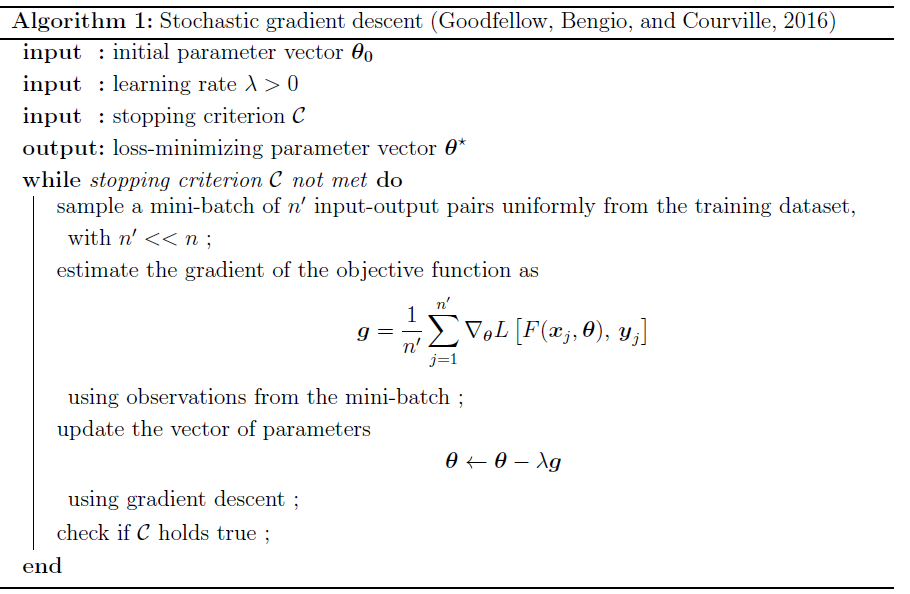
\includegraphics[width=0.7\linewidth]{DL on Macro model/Pascal et al 2024 Working paper/Reading Note/stochastic gradient descent algorithm.png}

\end{figure}
    
\end{frame}

\begin{frame}{Validation and Regularization}
The overall objective of DL technique is to provide algorithm that perform well on new inputs

\begin{itemize}
    \item Don't underfit: able to identify and learn the important properties of the data from the traning sample
    \item Don't overfit: not learned various idiosyncrasies of the training dataeset that will not generalize well to new inputs
    \item Broaderly: model should have the right capacity for the task force, i.e., the complexity is enough to represent the data but not overly complex. ==> the NN should have the right structure. This is validation
\end{itemize}
    
\end{frame}

\begin{frame}{DSGE model as minimization problem}
    \begin{enumerate}
        \item We describe the DSGE model 
        \item Transform it into the minimization problem 
        \item AiO operator
    \end{enumerate}
\end{frame}

\begin{frame}{DSGE model in short}
DSGE model is a dynamical system involving three kinds of variables
\begin{enumerate}
    \item Exogenous variables $z_t\in\mathbb{R}^{n_z}$ evolves according to Markov process
    $$
    z_{t} = Z(z_t-1, \epsilon_t)
    $$
    where $\epsilon_t\in\mathbb{R^{n_\epsilon}}$ is an i.i.d. innovation.
    $$
    Z: \mathbb{R}^{n_z}\times \mathbb{R}^{n_\epsilon}\to \mathbb{R}^{n_z}
    $$
    a \textbf{known} function
    \item Endogenous state variable $s_t\in\mathbb{R}^{n_s}$ is driven by the exogenous process and an endogenous control variable $c_t\in\mathbb{R}^{n_c}$, according to a \textbf{known} function
    $$
    S: \mathbb{R}^{n_z} \times \mathbb{R}^{n_s} \times \mathbb{R}^{n_c}\to \mathbb{R}^{n_s}
    $$
    $$
    s_{t+1} = S(z_t, s_t,c_t)
    $$
\end{enumerate}


    
\end{frame}
\begin{frame}{DSGE model in short}
\begin{itemize}
    \item Control variables solve some contrainted optimization problems. They verify $n_c$ number of first-order/equilibrium conditions of the form. (Equilibrium conditions--> constraints, first-order conditions --> optimization):
    $$
    \mathbb{E}_t f_j(\textcolor{blue}{z_t, s_t, c_t}, \textcolor{red}{z_{t+1}, s_{t+1}, c_{t+1}})=0,\quad j=1,\cdots, n_c
    $$
\end{itemize}
    
\end{frame}

\begin{frame}{DSGE in short}
Since the only source of the uncertainty is from $\epsilon_{t+1}$, which is implicitly contained in $z_{t+1}$, we can represent the first-order/equilibrium condition as

$$
\mathbb{E}_{\epsilon'}f_j(\textcolor{blue}{z, s, c}, \textcolor{red}{z', s', c'})=0,\quad j=1,\cdots, n_c
$$
where $\mathbb{E}_{\epsilon'}$ means taking expectation with respect to $\epsilon'$.
    
\end{frame}

\begin{frame}{Solution}
    Solving the model is to find a \textbf{time-invariant} decision rule, i.e., a function
    $$
    \sigma^*: \mathbb{R}^{n_z}\times \mathbb{R}^{n_s} \to \mathbb{R}^{n_c}
    $$
    such that $c=\sigma^*(z,s)$ satisfies all the first-order/equilibrium conditions, i.e.,
    $$
    \mathbb{E}_{\epsilon'}f_j(z, s, \textcolor{red}{\sigma^*(z,s)}, z', s', \textcolor{red}{\sigma^*(z',s')})=0,\quad j=1,\cdots, n_c
    $$
    for all possible $(z,s)\in\mathbb{R}^{n_z}\times\mathbb{R}^{n_s}$
\end{frame}

\begin{frame}{Parameterize the solution}
    Consider a family of parametric candidate decision rules
    $$
    S_\sigma = \{\sigma(\cdot;\theta):\theta\in\mathbb{R}^p\}
    $$
    indexed by the parameter vectors $\theta\in\mathbb{R}^p$. The most accurate approximation to the true decision rule contained in $S_\sigma$ is $\sigma(\cdot;\theta)$ function that best fits the first-order/equilibrium conditions.
\end{frame}

\begin{frame}{Minimization Problem}
    Use the MSE as the loss function, we can formulate it as a minimization problem:
    $$
    \sigma^*(z,s) = \arg\min_\theta \sum_{j=1}^{n_c} v_j \left[\mathbb{E}_{\epsilon'} f(z,s,\sigma(z,s;\theta), z',s',\sigma(z',s';\theta))\right]^2
    $$

    But this is only for the point $(z,s)$. We need this for all $(z,s)\in\mathbb{R}^{n_z}\times\mathbb{R}^{n_s}$
\end{frame}

\begin{frame}{Computation Complexity}
Since we need to solve the first-order/equilibrium condition for all possible $(z,s)\in\mathbb{R}^{n_z}\times\mathbb{R}^{n_s}$ numerically. This can be computationally demanding.\\
\\
One possible way to achieve high accuracy on a larger domain would be construct a solution on a grid of initial conditions.\\
\\
Maliar et al 2021 JMP propose an alternative approach which is more suitable for Monte Carlo simulation.\\
\\
They reformulate the first-order/equilibrium condition as an expectation function. Instead of a fixed grid, we assume that initial condition is drawn randomly from the domain on which we want the solution to be accurate.
\end{frame}

\begin{frame}{Maliar et al 2021 JMP}
This yields the following form:

$$
    \sigma^* = \arg\min_\theta \mathbb{E}_{(z,s)}\left\{\sum_{j=1}^{n_c} v_j \left[\mathbb{E}_{\epsilon'} f(z,s,\sigma(z,s;\theta), z',s',\sigma(z',s';\theta))\right]^2\right\}
    $$

But double expectation can also be computationally demanding. Maliar et al 2021 JMP introduce the AiO operator. 

\end{frame}


\begin{frame}{All-in-One (AiO) operator}
AiO operator combines the two expectations into single one. Using the following property
$$
[\mathbb{E}_{\epsilon} g(z,\epsilon)]^2 = [\mathbb{E}_{\epsilon_1} g(z,\epsilon_1)][\mathbb{E}_{\epsilon_2} g(z,\epsilon_2)] = \mathbb{E}_{(\epsilon_1, \epsilon_2)} g(z,\epsilon_1)g(z,\epsilon_2)
$$
where $z,\epsilon$ are random variables.  This transform 

    $$
    \bigg[\mathbb{E}_{\epsilon'} f(z,s,\sigma(z,s;\theta), z',s',\sigma(z',s';\theta))\bigg]^2
    $$
to

$$
\mathbb{E}_{(\epsilon_1, \epsilon_2)} \bigg[f_j(\cdots)\bigg|\epsilon = \epsilon_1\bigg] \bigg[f_j(\cdots)\bigg|\epsilon = \epsilon_2\bigg]
$$
\end{frame}

\begin{frame}{AiO}
    Since $(z,s)$ is independent of $(\epsilon_1,\epsilon_2)$, we can transform the minimization problem to

    $$
    \sigma^* = \arg\min_\theta \mathbb{E}_{(z,s,\epsilon_1,\epsilon_2)}\left\{\sum_{j=1}^{n_c} v_j \bigg[f(\cdots)\bigg|\epsilon = \epsilon_1\bigg]\bigg[f(\cdots)\bigg|\epsilon = \epsilon_2\bigg]\right\}
    $$

\end{frame}

\begin{frame}{Notation}
    Maliar et al 2021 JMP refer to this as Euler residual minimization. We can simplify the notation by letting $\omega:= (z,s,\epsilon_1, \epsilon_2)$, 
    \begin{itemize}
        \item $\omega:= (z,s,\epsilon_1, \epsilon_2)$, 
        \item $f_{j,i} = f_j(\cdots)|\epsilon= \epsilon_i$
    \end{itemize}
    Hence, we have
    $$
    \Xi(\theta) = \mathbb{E}_\omega\left[\sum_{j=1}^{n_c}v_j f_{j,1}(\omega;\theta)f_{j,2}(\omega;\theta)\right]:= \mathbb{E}_\omega g(\omega, \theta)
    $$
\end{frame}


\begin{frame}{DL solution step 1}
\begin{enumerate}
    \item Define an empirical counterpart to $\Xi(\theta)$
    $$
    \widehat{\Xi}(\theta) = \frac{1}{n}\sum_{j=1}^n g(\omega_i;\theta)
    $$
    given a \textbf{sample of artificial observations} $\{\omega_i\}_{i=1}^n$
    \item Define the set of candidate decision rule $S_\sigma$, i.e., choose the architecture of the neural networks. 
    \item Choose the initial parameter vector $\theta$
    \item Choose a stopping criteria $C$
\end{enumerate}
    
\end{frame}

\begin{frame}{DL solution step 2 - Learning Process}
\begin{enumerate}
    \item Given the current decision rule $\sigma(\cdot;\theta)$, simulate the model to produce artificial data $\{w_i\}_{i=1}^n$
    \item Update the parameter vector using stochastic gradient descent
    \item go to next step is the stopping criteria $C$ is satisfied, otherwise return to the beginning.
\end{enumerate}

    
\end{frame}


\begin{frame}{DL solution Step 3 - evaluation and validation}
\begin{enumerate}
    \item Evaluate the accurary of the candidate solution $\sigma(\cdot; \theta^*)$ on a new sample
    \item Stop if the solution is accurate; otherwise go back to the beginning and update the network architecture. 
\end{enumerate}
\end{frame}


\begin{frame}{Example Model}
\begin{itemize}
    \item Given initial capital stock $k_0$
    \item an exogenous process for TFP $a_t$
    \item Choose consumption $c_t$, capital $k_{t+1}$, labor $h_t$, investment $x_t$
    \item maximize the expected lifetime utility of a representative consumer
    $$
    \max_{\{c_t,k_{t+1}, h_t,x_t\}_{t=0}^\infty} \mathbb{E}_0\sum_{t=0}^\infty \beta^t [\eta \ln c_t + (1-\eta)\ln(1-h_t)]
    $$
\end{itemize}

\end{frame}

\begin{frame}{Model}
    $$
    \max_{\{c_t,k_{t+1}, h_t,x_t\}_{t=0}^\infty} \mathbb{E}_0\sum_{t=0}^\infty \beta^t [\eta \ln c_t + (1-\eta)\ln(1-h_t)]
    $$
    subject to 
\begin{align*}
    y_t &= c_t + x_t\\
    y_t &= a_tk_t^\alpha h_t^{1-\alpha}\\
    k_{t+1} &=(1-\delta) k_t + x_t\\
    \ln a_t &= \rho \ln a_{t-1} + \epsilon_t
\end{align*}
where $y_t$ is total output, $\beta\in(0,1)$ is the discount factor, $\eta\in(0,1)$ is a preference weight, $\alpha\in(0,1)$ is the capital share, $\delta\in(0,1)$ is the depreciation rate, $\rho\in(0,1)$ is the persistence of TFP, $\epsilon_t$  is iid Gaussian innovation with zero mean and variance $\sigma^2>0$. 
\end{frame}

\begin{frame}{First-order conditions}
$$
(1-\eta)c_th_t = \eta(1-\alpha) (1-h_t)y_t
$$
$$
1= \beta\mathbb{E}_t\frac{c_t}{c_{t+1}} \left[\alpha \frac{y_{t+1}}{k_{t+1}}+1-\delta\right]
$$
    
\end{frame}

\begin{frame}{First-order/equilibrium conditions}
    6 equations, 6 unknowns, no closed form solution
\begin{align*}
    y_t &= c_t + x_t\\
    y_t &= a_tk_t^\alpha h_t^{1-\alpha}\\
    k_{t+1} &=(1-\delta) k_t + x_t\\
    \ln a_t &= \rho \ln a_{t-1} + \epsilon_t\\
    (1-\eta)c_th_t &= \eta(1-\alpha) (1-h_t)y_t\\
    1&= \beta\mathbb{E}_t\frac{c_t}{c_{t+1}} \left[\alpha \frac{y_{t+1}}{k_{t+1}}+1-\delta\right]
\end{align*}
\end{frame}

\begin{frame}{Calibration}
\begin{itemize}
    \item yearly frequency
    \item $\alpha = 0.36$
    \item $\beta=0.96$
    \item $\delta=0.10$
    \item $\eta=0.33$
    \item $\rho=0.92$
    \item $\sigma_{\epsilon} = 0.014$
\end{itemize}
    
\end{frame}

\begin{frame}{Write the model in DL form}
We need to characterize
\begin{itemize}
    \item $\epsilon$, $z, s,c,Z,S,f$
    \item Only TFP shock $\implies n_\epsilon =1,\epsilon_t = \epsilon_t$
    \item only one exogenous variable $z_t = a_t$ and $n_z=1$
    \item only endogenous variables is capital $s_t=k_t$, $n_s=1$
    \item four control variables $c_t = (c_t, h_t,x_t, y_t)'$, $n_c=4$
\end{itemize}
    
\end{frame}

\begin{frame}{Write the model in DL form}
\begin{itemize}
    \item $Z$ is the law of motion for $a_t$, i.e.,
    $$
    \ln a_t = \rho \ln a_{t-1} + \epsilon_t
    $$
    \item $S$ is law of motion for capital $k_t$, i.e.,
    $$
    k_{t+1} &=(1-\delta) k_t + x_t
    $$
    \item $f$ are the four equilibrium conditions
\end{itemize}
    
\end{frame}

\begin{frame}{Write the model in DL form}
$$
f(z_t,s_t,c_t,z_{t+1}, s_{t+1}, c_{t+1}) = \begin{bmatrix}
    y_t-c_t-x_t\\
    y_t-\alpha_tk_t^\alpha h_t^{1-\alpha}\\
     (1-\eta)c_th_t-\eta(1-\alpha) (1-h_t)y_t\\
     \beta\mathbb{E}_t\frac{c_t}{c_{t+1}} \left[\alpha \frac{y_{t+1}}{k_{t+1}}+1-\delta\right]-1
\end{bmatrix}
$$
or in this simple model, we can simply the above into
$$
f(z_t,s_t,c_t, z_{t+1},s_{t+1},c_{t+1}) = \beta\frac{c_t}{c_{t+1}}\left(\alpha \frac{y_{t+1}}{k_{t+1}}+1-\delta\right)-1
$$
    
\end{frame}

\begin{frame}{DL objective function}
The DL objective function is
$$
\Xi(\theta) = \mathbb{E}_\omega f_1(\omega)f_2(\omega)
$$
where 
\begin{itemize}
    \item $\theta$ is the parameter vector
    \item $\omega= (z,s,\epsilon_1,\epsilon_2)$
    \item $f_i$ is the function $f$ evaluated at shock $\epsilon_i$
\end{itemize} 
    
\end{frame}

\begin{frame}{Network architecture and evaluation}
\begin{itemize}
    \item Depth: 1 or 2
    \item Width: 4 nodes, 16 nodes, 32 nodes
    \item activation function for input and hidden layer: hyperbolic tangent, ReLU, sigmoid
    \item activation function for output: sigmoid
    \item number of observations included in the mini-batch: 1, 10, 100, 1000
    \item learning algorithm: basic stochastic gradient descent, Adam algorithm of Kingma and Ba 2017
    \item Learning rate $\lambda$: 0.1, 0.0001 for Adam
    \item train the network with 5000 gradient iteration and measure the performance at every step
\end{itemize}
    
\end{frame}

\begin{frame}{Network architecture and evaluation}
Evaluate the accuracy of the neural network solution using the unit-free Euler equation error of Judd and Guu 1997 and Barillas and Fernandez-Villaverde 2007, defined as
$$
EEE(a,k) = 1- \left\{\beta \mathbb{E} \left[\frac{c}{c'}\left(\alpha \frac{y'}{k'}+1-\delta\right)\right]\right\}^{-1}
$$
with
\begin{itemize}
    \item $\phi = \sigma(a,k;\theta)$, $h = \eta(1-\alpha)/[\eta(1-\alpha)+(1-\eta)\phi]$
    \item $c= \phi a k^\alpha h^{1-\alpha}, k' = (1-\delta)k+(1-\phi)ak^\alpha h^{1-\alpha}$
    \item $a' = \exp[\rho \ln(a)+\epsilon']$, $\phi' = \sigma(a',k';\theta)$, $h' = \eta(1-\alpha)/[\eta(1-\alpha)+(1-\eta)\phi'] $
    \item $y'=a'(k')^\alpha (h')^{1-\alpha}$, $c'=\phi' y'$
    \item All model equations are exactly verified conditional on $\phi$, except for the Euler equations.
\end{itemize}
    
\end{frame}

\begin{frame}{Euler equation error}
\begin{itemize}
    \item All model equations are exactly verified conditional on $\phi$, except for the Euler equations. This is why the EEE statistic provides a summary accuracy measure for the DL solution.
    \item It has a simple economic interpretation: a value of 0.01 implies that agents make a mistake of $\$1$ for every $\$100$ spent. 
\end{itemize}
    
\end{frame}

\begin{frame}{Computation Details}
\begin{itemize}
    \item When computing the loss function $\Xi(\theta)$ and the $EEE(a,k)$, we sample productivity $\ln (a)$ from its ergodic distribution $N(0,\sigma^2/(1-\rho^2))$ and capital $k$ from a normal distribution $N(\mu_k, \sigma_k^2)$, where $\mu_k$ and $\sigma_k^2$ denote the average and the standard deviation of $k$ implied by the first-order approximation of the model. 
\end{itemize}
    \textbf{Remark:} They checked ex post that these bounds provide good coverage of the ergodic set, based on simulation from the DL solution. For more complex models, an alternative would be to add a loop to the algorithm in order to draw the endogenous state variable from its simulated ergodic distribution, while checking for the convergence of the distribution. This would slow down the execution time. 
\end{frame}

\begin{frame}{Initialize the parameter vector}
To initialize the parameter vector $\theta$, we use the closed-form solution that the model admits when $\delta=1$,i.e., with full capital depreciation. In practice, this solution is $\phi=1-\alpha\beta$ and we run an initial training step tp have the network learn this value for various productivity-capital draw $(a,k)$. An alternative possibility would be to use the standard first-order approximation of the policy rule to initialize $\theta$.
    
\end{frame}

\end{document}
